\chapter{SPN Scanning-Service Discovery without Network Port Scanning}

The best way to discover services in an Active Directory environment is through what I call “SPN Scanning.”

The primary benefit of SPN scanning for an attacker over network port scanning is that SPN scanning doesn’t require connections to every IP on the network to check service ports. SPN scanning performs service discovery via LDAP queries to a Domain Controller. Since SPN queries are part of normal Kerberos ticket behavior, it is difficult, if not infeasible to detect, while netowkr port scanning is pretty obvious.

Service Principal Names (SPNs) are required for discovery of services that leverage Kerberos authentication.


From the Microsoft Kerberos specification:

An SPN is a string of the following format. For more information on the <alphanum> element, see [RFC2396] section 1.6.
SPN = serviceclass “/” hostname [“:”port] [“/” servicename]
serviceclass = alphanum
servicename = alphanum
Where:
serviceclass is a string that identifies the class of the service, such as “www” for a Web service or “ldap” for a directory service.
hostname ([RFC2396] section 3.2.2) is a string that is the name of the system. This SHOULD be the fully qualified domain name (FQDN).
port ([RFC2396] section 3.2.2) is a number that is the port number for the service.

The servicename segment is a string that is the distinguished name (DN), objectGuid, Internet host name, or fully qualified domain name (FQDN) for the service.
An application can supply a name of the form “RestrictedKrbHost/<hostname>” when its callers have provided the hostname but not the correct SPN for the service. Applications SHOULD NOT use “RestrictedKrbHost/<hostname>” due to the security considerations in section 5.1.2. Applications calling GSS-API directly MUST provide a target name which SHOULD be an SPN<28> for their service applications for Kerberos authentication.

Some of the more interesting services and example SPNs:

SQL servers, instances, ports, etc.
MSSQLSvc/adsmsSQLAP01.adsecurity.org:1433
Exchange
exchangeMDB/adsmsEXCAS01.adsecurity.org
RDP
TERMSERV/adsmsEXCAS01.adsecurity.org
WSMan / WinRM / PS Remoting
WSMAN/adsmsEXCAS01.adsecurity.org
Hyper-V Host
Microsoft Virtual Console Service/adsmsHV01.adsecurity.org
VMWare VCenter
STS/adsmsVC01.adsecurity.org


Here’s the result of a PowerShell script that performs SPN scanning for Microsoft SQL Servers.
\begin{figure}
    \centering
    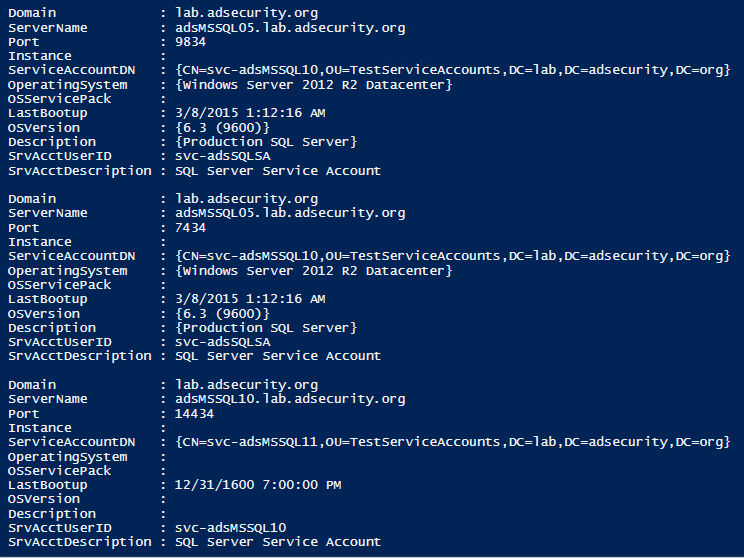
\includegraphics[width=0.75\linewidth]{spnscan1.png}
    \caption{Service Principal Name (SPN) Scan}
    \label{fig:placeholder}
\end{figure}
